\documentclass[a4paper,12pt,twoside]{hmcpset}
\usepackage[utf8]{inputenc}
\usepackage[english]{babel}
\usepackage{fancyhdr}
\usepackage[margin=1in]{geometry}
\usepackage{graphicx}
\usepackage{amsmath}
\usepackage{mathtools}
\usepackage[mathscr]{euscript}
%\newcommand*{\ms}[1]{\ensuremath{\mathscr{#1}}}
\usepackage{lmodern} % math, rm, ss, tt
\usepackage[T1]{fontenc} 
\usepackage{tikz}
\usepackage{caption}


\pagestyle{fancy}
\fancyhf{}
\rhead{Spring 2019}
\chead{Section 6}
\lhead{\vspace{5mm} Math 147 Topology}
\rfoot{Page \thepage}
\linespread{1.3}
 

\renewcommand{\headrulewidth}{2pt}
\renewcommand{\footrulewidth}{2pt}

\graphicspath{ {./figures_theorems/} } 

% info for header block in upper right hand corner
\begin{document}

\section*{Chapter 6\\ Countable Features of Spaces: Size Restrictions}


\begin{exercise}[Exercise 6.1]
    Show that $A$ is dense in $X$ if and ony if every 
    non-empty open set of $X$ contains a point of $A$.
\end{exercise}

\begin{solution}
First we prove the forward direction. Suppose that $A$ is a dense subset in 
$X$. Then by definition, $\overline{A} = X$. Thus every point of $X$ 
is a limit point of $A$, which means that for every point $p \in X$ and 
every open set $U$ which contains $p$ we see that 
$$
(U - \{p\})\cap A \ne \emptyset.
$$
Since this holds for all $p \in X$, we see that every open set in $X$ must 
contain points in $A$, which proves this direction.

\begin{figure}[h!]
    \centering
    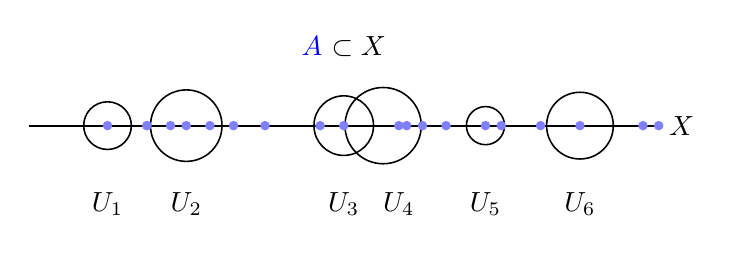
\begin{tikzpicture}
        \draw[black, thick] (0, 0) -- (8, 0) node[anchor=west] {$X$}
        node at (4, 1) {\color{blue}$A$ \color{black}$\subset X$};
        \draw[line width=.2mm,color=black] (1,0) circle (2ex) node at
        (1,-1) {$U_1$};
        \draw[line width=.2mm,color=black] (2,0) circle (3ex)node at
        (2,-1) {$U_2$};
        \draw[line width=.2mm,color=black] (4,0) circle (2.5ex)node at
        (4,-1) {$U_3$};
        \draw[line width=.2mm,color=black] (4.5,0) circle (3.2ex)node at
        (4.7,-1) {$U_4$};
        \draw[line width=.2mm,color=black] (5.8,0) circle (1.6ex)node at
        (5.8,-1) {$U_5$};
        \draw[line width=.2mm,color=black] (7,0) circle (2.8ex)node at
        (7,-1) {$U_6$};

        \filldraw [blue!50] (1,0) circle (1.5pt);
        \filldraw [blue!50] (2,0) circle (1.5pt);
        \filldraw [blue!50] (3,0) circle (1.5pt);
        \filldraw [blue!50] (4,0) circle (1.5pt);
        \filldraw [blue!50] (5,0) circle (1.5pt);
        \filldraw [blue!50] (6,0) circle (1.5pt);
        \filldraw [blue!50] (7,0) circle (1.5pt);
        \filldraw [blue!50] (8,0) circle (1.5pt);
        \filldraw [blue!50] (1.5,0) circle (1.5pt);
        \filldraw [blue!50] (2.6,0) circle (1.5pt);
        \filldraw [blue!50] (3.7,0) circle (1.5pt);
        \filldraw [blue!50] (5.3,0) circle (1.5pt);
        \filldraw [blue!50] (4.8,0) circle (1.5pt);
        \filldraw [blue!50] (7.8,0) circle (1.5pt);
        \filldraw [blue!50] (6.5,0) circle (1.5pt);
        
        \filldraw [blue!50] (4.7,0) circle (1.5pt);
        \filldraw [blue!50] (2.3,0) circle (1.5pt);
        \filldraw [blue!50] (5.8,0) circle (1.5pt);
        \filldraw [blue!50] (1.8,0) circle (1.5pt);
        \filldraw [blue!50] (1.5,0) circle (1.5pt);
    \end{tikzpicture}
    \begin{caption}\\
        Here we see the set \color{blue}$A$ \color{black}is a dense subset in $X$. The
        sets $U_1, \dots U_6$ denote arbitrary open sets in $X$.
    \end{caption}
\end{figure}


Now suppose that every nonempty open set of $X$ contains a point of $A$. 
Then this means that for any $p \in X$, any open set $U$ containing $p$ 
must also contain a point in $A$. By definition, this is a limit point.
Since $p$ was an arbitrary point of $x$, we must have that every element 
of $X$ is a limit point of $A$. Therefore, we must have that 
$\overline{A} = X$, which finishes the proof in this direction. 
\end{solution}

\begin{exercise}[Exercise 6.2]
Show that $\mathbb{R}_{\text{std}}$ is separable.
With which of the topologies on $\mathbb{R}$ that you have studied is
$\mathbb{R}$ not separable?
\end{exercise}

\begin{solution}
Observe that a countable dense subset in $\mathbb{R}_{\text{std}}$ is the 
set of rationals. This is because every nonempty open set of $\mathbb{R}$
on the standard topology contains points of $\mathbb{Q}$. By our previous 
exercise, this allows us to conclude that $\mathbb{Q}$ is dense in $\mathbb{R}$.
Since the rationals are countable, this in total allows us to conclude that 
$\mathbb{R}_{\text{std}}$ has a countable dense subset, and is therefore 
separable by definition. \\
However, this wouldn't hold for the discrete 
topology on $\mathbb{R}$, since it does not have a countable dense subset 
with this topology. The countable complement is also not separable, since 
every open set in the topology must be uncountable and hence finding a 
countable but dense subset of $X$ is impossible.
\end{solution}

\begin{exercise}[Exercise 6.4]
Find a separable space that contains a subspace that 
is not separable in the subspace topology.
\end{exercise}

\begin{solution}
\noindent \textit{Lemma.} An uncountable set with the discrete topology is not separable. 
\\
\\
\textit{Proof}. For the sake of contradiction suppose that $X$ is
uncountable and is separable under the discrete topology. Then there
exists a countable dense set $A$ such that $\overline{A} = X$.
However, since $X$ has the discrete topology, we know that $A =
\overline{A} = X$; a contradiction since $A$ is countable while $X$ is
uncountable. Thus $X$ is not separable under the discrete topology. 
\\
\\
Now consider a topology on an uncountable set $X$ given by 
\[
    \mathscr{T} = \{ \emptyset\} \cup \{U \subset X \}_{p \in X}
\]
where $p \in X$. Observe that $\{p\}$ is dense in this set since every
open set in $\mathscr{T}$ contains $\{p\}$ by construction. Since
$\{p\}$ is countable and dense, $X$ is separable on this topology. 

Consider the subspace $X - \{p\}$. For any $U \subset (X - \{p\})$, we
see that $U \cup \{p\} \subset \mathscr{T}$, so that $U$ is open in $X
- \{p\}$. Thus every subset of $X - \{p\}$ is open, which implies that
this is an uncountable discrete space. However, we know that an
uncountable discrete space is not separable, so that $X - \{p\}$ is
not separable.
\end{solution}

\noindent
\textbf{Presented in Class ?}\\
\begin{problem}[Theorem 6.5]
    If $X$ and $Y$ are separable spaces, then $X \times Y$ is separable.
\end{problem}

\begin{proof}
    Suppose $X$ or $Y$ are separable spaces. Then there exist countable sets 
    $A$ and $B$ such that $\overline{A} = X$ and $\overline{B} = Y$. 
    Using the fact that $\overline{A} \times \overline{B} = \overline{A \times B}$,
    we see that
    $$
    \overline{A \times B} = \overline{A} \times \overline{B} = X \times Y.
    $$
    Thus $A \times B$ is dense in $X \times Y$. But also observe that 
    $A \times B$ is countable, since we can form a bijection between $A 
    \times B$ and $A$ or $B$ (namely the projection function). Thus $X \times Y$
    must be separable because it contains a countable dense subset, which is 
    what we set out to show.

\begin{figure}[h!]
    \centering
    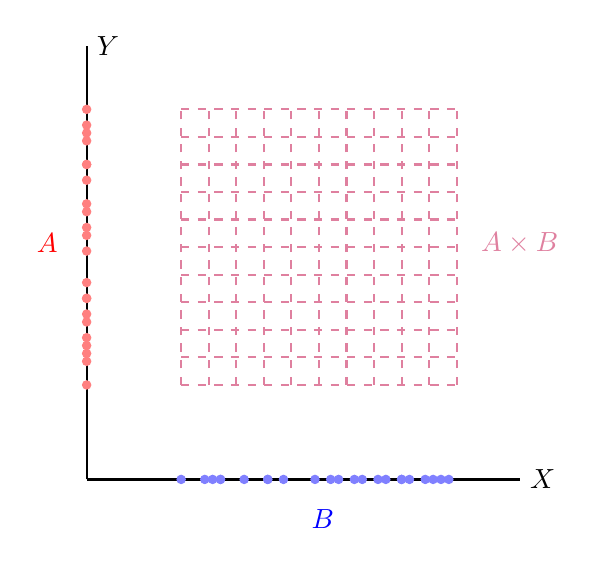
\begin{tikzpicture}
        \draw[black, thick] (-0.5, -0.5) -- (5, -0.5) node[anchor=west] {$X$};
        \draw[black, thick] (-0.5, -0.5) -- (-0.5, 5) node[anchor=west] {$Y$};

        \filldraw [blue!50] (1,-0.5) circle (1.5pt);
        \filldraw [blue!50] (2,-0.5) circle (1.5pt);
        \filldraw [blue!50] (3,-0.5) circle (1.5pt);
        \filldraw [blue!50] (4,-0.5) circle (1.5pt);
        \filldraw [blue!50] (1.2,-0.5) circle (1.5pt);
        \filldraw [blue!50] (3.5,-0.5) circle (1.5pt);
        \filldraw [blue!50] (3.3,-0.5) circle (1.5pt);
        \filldraw [blue!50] (3.8,-0.5) circle (1.5pt);
        \filldraw [blue!50] (1.5,-0.5) circle (1.5pt);
        \filldraw [blue!50] (2.6,-0.5) circle (1.5pt)
        node at (-1, 2.5) {\color{red}$A$};
        \filldraw [blue!50] (2.4,-0.5) circle (1.5pt);
        \filldraw [blue!50] (2.9,-0.5) circle (1.5pt);
        \filldraw [blue!50] (1.8,-0.5) circle (1.5pt);
        \filldraw [blue!50] (2.7,-0.5) circle (1.5pt);
        \filldraw [blue!50] (3.5,-0.5) circle (1.5pt);
        
        \filldraw [blue!50] (0.7,-0.5) circle (1.5pt);
        \filldraw [blue!50] (1.2,-0.5) circle (1.5pt);
        \filldraw [blue!50] (1.1,-0.5) circle (1.5pt);
        \filldraw [blue!50] (3.9,-0.5) circle (1.5pt);
        \filldraw [blue!50] (1.8,-0.5) circle (1.5pt);
        \filldraw [blue!50] (4.1,-0.5) circle (1.5pt);
        \filldraw [blue!50] (3.2,-0.5) circle (1.5pt);
        \filldraw [blue!50] (3.6,-0.5) circle (1.5pt);

        %%%%%%%%%%%%%%%%%%%%%%%%%%%%%%
        \filldraw [red!50] (-0.5,1) circle (1.5pt);
        \filldraw [red!50] (-0.5,2) circle (1.5pt);
        \filldraw [red!50] (-0.5,3) circle (1.5pt);
        \filldraw [red!50] (-0.5,4) circle (1.5pt);
        \filldraw [red!50] (-0.5,1.2) circle (1.5pt);
        \filldraw [red!50] (-0.5,3.5) circle (1.5pt);
        \filldraw [red!50] (-0.5,3.3) circle (1.5pt);
        \filldraw [red!50] (-0.5,3.8) circle (1.5pt);
        \filldraw [red!50] (-0.5,1.5) circle (1.5pt);
        \filldraw [red!50] (-0.5,2.6) circle (1.5pt)
        node at (2.5, -1) {\color{blue} $B$};
        \filldraw [red!50] (-0.5,2.4) circle (1.5pt);
        \filldraw [red!50] (-0.5,2.9) circle (1.5pt);
        \filldraw [red!50] (-0.5,1.8) circle (1.5pt);
        \filldraw [red!50] (-0.5,2.7) circle (1.5pt);
        \filldraw [red!50] (-0.5,3.5) circle (1.5pt);
        
        \filldraw [red!50] (-0.5,0.7) circle (1.5pt);
        \filldraw [red!50] (-0.5,1.3) circle (1.5pt);
        \filldraw [red!50] (-0.5,1.8) circle (1.5pt);
        \filldraw [red!50] (-0.5,1.1) circle (1.5pt);
        \filldraw [red!50] (-0.5,1.6) circle (1.5pt);
        \filldraw [red!50] (-0.5,4.2) circle (1.5pt);
        \filldraw [red!50] (-0.5,3.9) circle (1.5pt);

        %%%%%%%%%%%%%%%%%%%%%%%%%%%%%%
        \draw[purple!50, step=0.35cm, thick, dashed] (0.7,0.7) grid
        (4.2,4.2) node at (5, 2.5) {\color{purple!50} $A \times B$};        
    \end{tikzpicture}
    \caption{Here in this picture, we see that if $A$ and $B$ are
    countable dense subsets, then their product forms a countable
    dense subset.}
\end{figure}



\end{proof}

\begin{problem}[Theorem 6.6]
    The space $2^{\mathbb{R}}$ is separable.
\end{problem}

\begin{proof}
    Consider 
    \begin{align*}
        A = \Big\{f \in 2^\mathbb{R}: \bigcup_{i = 1}^n [p_i, q_i] | p_i, q_i \in \mathbb{Q} \Big| \forall x \in [p, q], f(x) = 1, x \notin [p_i, q_i], f(x) = 0\}\\
        \bigcup  \Big\{f \in 2^\mathbb{R}: \bigcup_{i = 1}^n [p_i, q_i] | p_i, q_i \in \mathbb{Q} \Big| \forall x \in [p, q], f(x) = 0, x \notin [p_i, q_i], f(x) = 1\}
    \end{align*}
    that is, we only consider intervals $[p, q]$, which have rational
    endpoints, and finitely union them. 
    To construct the points $f$ in our set, we assign either a 1 or a 0
    to $f(x)$ when $x$ lies in any of the finite intervals $[p_i,
    q_i]$. (This actually doesn't
    have to be done with $\mathbb{Q}$, but rather any set dense in
    $\mathbb{R}$.) 
    \\
    \\
    Theorem 2.14 guarantees that this is an at most countable
    set. Observe that our set is really a subset of all finite subsets
    of $\mathbb{Q}$, which itself is a countable set.
    \\
    \\
    Observe that this set is dense in $2^\mathbb{R}$. Consider an open set 
    \[
        U = \{f \in 2^\mathbb{R} : f(a_1) = \delta_1, \dots , f(a_n) = \delta_n\}
    \]
    where $\delta_1, \dots, \delta_n \in \{0, 1\}$. Then the point $f
    \in 2^\mathbb{R}$ such that $f(a_i) = \delta_i, f(x) = 0$
    otherwise, is a point in $U$. Call this point $y$.
    \\
    \\   
    Since $\mathbb{R}$
    is normal, there exist
    disjoint closed neighborhoods $[p_i, q_i]$ 
    such that $a_i \in [p_i, q_i]$ Then observe that the set 
    \[
        \bigcup_{i = 1}^n\{f \in 2^\mathbb{R} : f(x) = \delta_i \text{ if } x \in [p_i, q_i], f(x) = 0 \text{ otherwise}  \}  
    \] 
    is (1) a subset of $A$ and (2) contains $y$. Therefore, $A$ and
    $U$ have a nonempty intersetion, and since $U$ was an arbitrary
    open set of $2^\mathbb{R}$, we see that $A$ is dense in
    $2^\mathbb{R}$. Since it is also countable, we have that
    $2^\mathbb{R}$ is separable, as desired.
\end{proof}

\begin{problem}[Theorem 6.9]
    Let $X$ be a $2^{\text{nd}}$ countable space. Then $X$ is separable.
\end{problem}

\begin{proof}
    Let $p_i$ be some point of $B_i$, $i \in \mathbb{N}$, where $B_i$ is a basic open set 
    from our countable basis. Then for any open set $V$ of $X$, 
    we know that $V$ will intersect $\{p_i\}_{i \in \mathbb{N}}$ 
    since by definition $V$ must contain some basic open set $B_i$ for 
    which $p_i \in B_i$. Thus by Exercise 6.1, $\{p_i\}$ is dense, and 
    since it's countable we have that $X$ is separable.
\end{proof}

\begin{exercise}[Exercise 6.10]
\begin{itemize}
\item[1.] The space $\mathbb{R}_{\text{std}}$ is $2^{\text{nd}}$
countable (and hence separable).

\item[2.] The space $\mathbb{R}_{\text{LL}}$ is separable but not
$2^\text{nd}$ countable.

\item[3.] The space $\mathbb{H}_{\text{bub}}$ is seprarble but not
$2^\text{nd}$ countable.
\end{itemize}
\end{exercise}

\begin{solution}
    \begin{itemize}
        \item[1.] 
        Consider the open set $(a, b)$. Then observe that 
        \[
           \left(\bigcup\limits_{p \in \mathbb{Q}, a \le p}(p, \infty)\right) 
           \cap
           \left(\bigcup\limits_{q \in \mathbb{Q}, q \le b}(\infty, q)\right)
           = 
           (a, b).  
        \]
        Therefore, we can generate $(a, b)$ by open sets with rational
        endpoints, which shows that $\mathbb{R}$ has a countable basis. 
        Specifically, the family of open sets $\{(p,q) : p, q \in
        \mathbb{Q}\}$ forms a countable basis for
        $\mathbb{R}_\text{std}$, so that by definition
        $\mathbb{R}_\text{std}$ is $2^\text{nd}$ countable.
    
        \item[2.] 
        By Exercise 6.2, we found that
        $\mathbb{R}_\text{std}$ is separable since the rationals form a
        countable, dense subset in $\mathbb{R}_\text{std}$. Thus every set
        $(a, b)$ contains a rational.
        However, $(a, b) \subset [a, b)$, which
        which means that every set $[a, b)$ must also intersect the
        rationals. By Exercise 6.1, we can then conclude that the
        rationals are dense in $\mathbb{R}_{\text{LL}}$, and since they
        are countable this implies that $\mathbb{R}_\text{LL}$ is
        separable.
        
        \item[3.] Observe that the positive rationals $\mathbb{Q}^+$ form
        a dense set of $\mathbb{R}^+\cup{0}$. That is, any set with $(a, b)$ with
        $a, b \ge 0$ must contain a rational. By Theorem 6.5, we can then
        conclude that $(\mathbb{Q}^+)^2$ is dense in $(\mathbb{R}^+)^2$,
        and $\mathbb{Q}^+)^2$ is clearly countable. Thus by definition
        $(\mathbb{R}^+)^2$ is separable. 
    
        However, observe that this is not $2^{nd}$ countable. Observe that
        if we are to cover this space, we need to cover the $x$-axis.
        But every point on the $x$ axis needs an individual sticky
        bubble to cover it, and since there are an uncountable number of
        such $x$, it would be impossible to cover all of them with a
        countable number of sticky bubbles. Therefore this space is not
        $2^{nd}$ countable. 
    
        
    \end{itemize}
\end{solution}

\begin{problem}[Theorem 6.11]
    Every uncountable set in a $2^{\text{nd}}$ countable space has a limit point. 
\end{problem}

\begin{proof}
    Suppose we have an uncountable set $A$ in $X$, and for the sake of
    contradiction suppose that $U$ has no limit points. Then every point
    of $A$ is an isolated point, which means that there exists an open set 
    $U$ such that $U \cap A = \{p\}$ for all $p \in A$. Note that
    for every such $U$ there exists a $B$ basic open set such that $B \subset U$.
    Thus $p \in B \subset U$. 
    However, there are only countably many basic open sets, while an uncountable 
    number of $p \in A$, which is a contradiction since we cannot contain an uncountable 
    number of points with a countable number of basic open sets. Thus $A$ 
    must have a limit point, which is what we set out to show. 
\end{proof}

\begin{problem}[Theorem 6.14]
    Let $X$ be $2^\text{nd}$ countable. Then $X$ is $1^\text{st}$
    countable. 
\end{problem}

\begin{proof}
    Let $X$ be a $2^{\textrm{nd}}$ countable space and $x \in X$. 
    Then $X$ has a
    countable basis $\mathscr{B}$. 
    Consider the set $\mathscr{B}_x$ of all 
    $B \in \mathscr{B}$ such that $x \in B$. 
    Since $\mathscr{B}$ is a basis, we know that for any open set $U$
    containing $x$ there exists a $B_x \in \mathscr{B}$ such that 
    \[
        p \in B_x \subset U.
    \]  
    But $p \in B_x$ so $B_x \in \mathscr{B}_x$. Therefore, $\mathscr{B}_x$ is a
    neighborhood basis of $x$. However, $\mathscr{B}_x \subset
    \mathscr{B}$ so $\mathscr{B}_x$ is countable.
    Therefore, every point of $x$ as countable neighborhood basis
    so it is a $1^{\textrm{st}}$ countable space. 
\end{proof}

\begin{problem}[Theorem 6.15]
    If $X$ is a topological space, $p \in X$, and $p$ has a countable
    neighborhood basis, then $p$ has a nested countable neighrborhood
    basis.
\end{problem}

\begin{proof}
    Let $\mathscr{B}$ be the countable neighborhood basis for $p$.
    Observe that for $B \in \mathscr{B}$, (1) $p \in B$ and (2) $B$ is
    an open set, so by Theorem 3.3 we must be able to contain $p$ in
    some neighborhood $U$ such that $p \in U \subset B$. By the
    defintion of a neighborhood basis, there must exist another $B'
    \in \mathscr{B}$ such that $p \in B' \subset U$. Hence, for every
    $B \in \mathscr{B}$, there exists an element $B' \in \mathscr{B}$
    such that 
    \[
      p \in B' \subset B.  
    \]
    Since $\mathscr{B}$ is countable, we can construct an at most
    countable set of nested open sets which form a neighborhood basis
    of $p$. Thus $p$ has a nested countable neighborhood basis as desired.
\end{proof}


\begin{problem}[Theorem 6.18]
    Suppose $x$ is a limit point of the set $A$ in a $1^{\text{st}}$
    countable space $X$. Then there is a sequence of points $\{a_i\}
    _{i \in \mathbb{N}}$ in $A$ that converges to $x$.     
\end{problem}

\begin{proof}
    Since $x$ is a limit point of $A$, for every open set $U$ such
    that $x \in U$ we have that $(U - \{x\}) \cap A \ne \emptyset$.
    Since $x$ is also a point in a first countable space, it has a
    countable neighborhood basis. By Theorem 6.15, $x$ must therefore
    also have a nested countable neighborhood basis $\mathscr{B}$. 
    \\
    \\
    Since $\mathscr{B}$ is countable, 
    we can write $\mathscr{B} = \{B_1, B_2, \dots \}$.
    Let $i \in \mathbb{N}$.
    Now since each $B_i\in \mathscr{B}$ 
    must contain some point $a_i \in A$, $a_i \ne x$, any open set of
    $x$ will contain some $a_i$ such that $a_i \in B_i \subset U$.
    Thus we must have that $\{a_i\}_{i \in \mathbb{N}}$ to be a
    sequence of points of $A$ which converges to $x$.
\end{proof}


\end{document}
